\documentclass{article}
\usepackage{graphicx}


\PassOptionsToPackage{numbers}{natbib}


% ready for submission
\usepackage[final]{neurips_2023}

\usepackage{amsmath,amsfonts,amssymb,amsthm}

% to compile a preprint version, e.g., for submission to arXiv, add add the
% [preprint] option:
%     \usepackage[preprint]{neurips_2023}


% to compile a camera-ready version, add the [final] option, e.g.:
%     \usepackage[final]{neurips_2023}


% to avoid loading the natbib package, add option nonatbib:
%    \usepackage[nonatbib]{neurips_2023}


\usepackage[utf8]{inputenc} % allow utf-8 input
\usepackage[T1]{fontenc}    % use 8-bit T1 fonts
\usepackage[hidelinks]{hyperref}       % hyperlinks
\usepackage{url}            % simple URL typesetting
\usepackage{booktabs}       % professional-quality tables
\usepackage{nicefrac}       % compact symbols for 1/2, etc.
\usepackage{microtype}      % microtypography
\usepackage{xcolor}         % colors
\usepackage{cleveref}
\newtheorem{theorem}{Theorem}[section]
\newtheorem{lemma}[theorem]{Lemma}
\newtheorem{proposition}[theorem]{Proposition}
\theoremstyle{definition}
\newtheorem{definition}[theorem]{Definition}
\newtheorem{example}[theorem]{Example}

\title{COMPSCI 683 Project Proposal}


% The \author macro works with any number of authors. There are two commands
% used to separate the names and addresses of multiple authors: \And and \AND.
%
% Using \And between authors leaves it to LaTeX to determine where to break the
% lines. Using \AND forces a line break at that point. So, if LaTeX puts 3 of 4
% authors names on the first line, and the last on the second line, try using
% \AND instead of \And before the third author name.


\author{%
  Erin Song\\
  \texttt{esong@umass.edu} \\
  \And
  Harold Thidemann\\
  \texttt{hthidemann@umass.edu} \\
  \And
  Shubhang Vagvala\\
  \texttt{svagvala@umass.edu} \\
  \And
  Jiaqi Ye\\
  \texttt{jiaqiye@umass.edu} \\
}


\begin{document}


\maketitle


\begin{abstract}
Our project explores how to solve a Nurikabe puzzle of varying board sizes. The puzzle is a binary determination puzzle that is NP-complete, 
meaning that the larger the board size, and exhaustive search would take a long time. We approach this problem as a Constraint Satisfaction 
Problem (CSP) and use --(insert algorithm solution)-- to solve it. We find that --(insert relevant results and conclusions)--. 
\end{abstract}

\section{Introduction}\label{sec:intro}
Nurikabe puzzles were developed in Japan and published in alogic puzzle magazine from Nikoli in 1991. The puzzle consists of a grid board 
where each cell can have one of three states. Each cell can be either black, white or contain a number. The rules are as follows:
\begin{enumerate}
    \item You cannot fill in cells containing numbers.
    \item A number tells the number of continuous white cells. Each area of white cells contains only one number in it and they are separated by black cells.
    \item The black cells are linked to be a continuous wall.
    \item Black cells cannot be linked to be 2×2 square or larger.
\end{enumerate}

Figure 1 shows an example puzzle along with its solution.  \\

\begin{figure}[h]
    \centering
    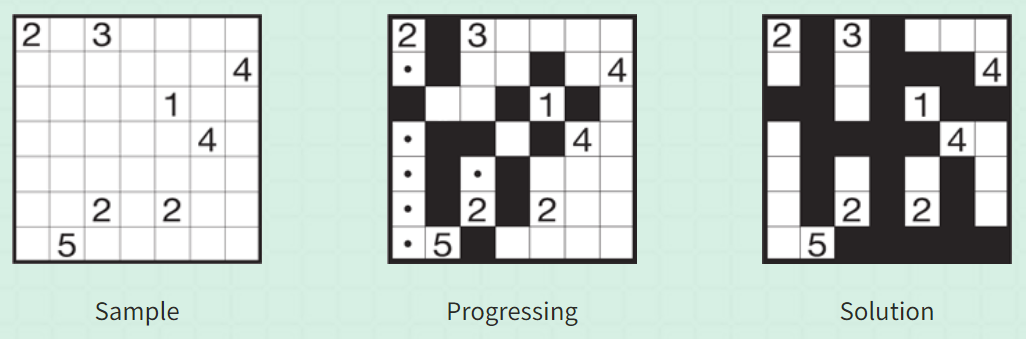
\includegraphics[width=0.75\textwidth]{./images/example.png} \\
    \caption{A Nurikabe Puzzle and its Solution}
\end{figure}
\subsection{Our Contributions}\label{sec:contrib}
We meet weekly to discuss the work we've done the past week and our goals for next week.

\begin{enumerate}
    \item Erin Song: Developed a way to visually represent game boards, wrote the intro and rules of the game, and will develop a method to check if a solution is correct.
    \item Harold Thidemann: Worked on code to generate data set of boards, will write the formal mathematical definitions and perform data analysis. 
    \item Shubhang Vagvala: Worked on code to make an interactive way to play Nurikabe and will do testing on the algorithm(s).
    \item Jiaqi Ye: Worked on code to generate data set of boards, reviewed related papers, and will develop algorithm(s) for solving Nurikabe.
\end{enumerate}

We plan on using the information from the related works section to develop an algorithm, or just picking one of them.

\subsection{Related Work}\label{sec:related}
Here is what we have found so far:

\hyperlink{https://theses.liacs.nl/pdf/18-JohanGroenen.pdf}{Johan Groenen} explains how to solve all solvable puzzles and check for unique solvability using brute force algorithms, extended with backtracking and optimizations. The algorithm expands islands recursively, each time adding a cell from an island’s neighborhood to itself, and then updating the neighborhood. If the island is full, the next island is expanded. If there is no next island, we check if there are no pools and only one stream (which would make it a solution). You can reduce the search time by not allowing expansion to cells that have been tried earlier.
\begin{itemize}
  \item Can also check if there are pools in unreachable areas of the puzzle; if so, there’s no solution and there is no need to keep checking it.
  \item There are two possible ways to generate puzzles. The first method is to generate all possible solutions, throw away all solutions containing pools and/or zero or multiple streams, create all corresponding puzzles by placing numbers in every way possible, and select all puzzles that appear only once in the generated set (which means they have only one solution). The second method is to generate all puzzles and check them for correctness. No two pivots can be neighbors and there is a maximum number of white cells, so it’s possible to skip a lot of configurations.
\end{itemize}

\hyperlink{http://www.spenceryoungcs.com/nurikabeGA.html}{Spencer Young et al.} developed a genetic algorithm solver for Nurikabe which can solve 5x5 Nurikabe problems in approx. 1 second. The solver uses all the traditional properties of genetic algorithms, such as population, mating pool, elitism, mutation, and breeding.

\hyperlink{https://dl.acm.org/doi/10.1145/3319619.3338470}{Martyn Amos et al.} made a Nurikabe solver using Ant Colony Optimization. 
\begin{itemize}
  \item At each iteration, a number of “ants” are given a local copy of the game board. Each ant constructs a solution.
  \item Each ant constructs a set of possible candidate cells starting from the “seed” of an island (a number on the grid). Candidate cells are initially the cells around the seed, and we prune cells that violate game constraints (remove any cell that cuts off the stream, remove any cell that is adjacent to an existing island, etc). Each ant will move on to the next “seed” until a complete solution is made.
  \item Then select the best performing ant (“according to a cost function which counts how many constraints are broken”), update the global pheromone matrix (future ants are then biased towards these “better” cells), and then “best value evaporation” operator is applied.
\end{itemize}

\hyperlink{https://dl.acm.org/doi/pdf/10.5555/3447286.3447294}{Paul Bass et al.} took a scattered neighborly approach to solving Nurikabe. The method combines scatter search and variable neighorhood search. 
\begin{itemize}
    \item Overview: generate a set of diverse (potential / partial) solutions using scatter search, selects the fittest subset of solutions, searches the space around the solutions to find the final correct, solved puzzle using VNS made up of four neighborhoods.
    \item Neighborhoods: Surplus island swap, unifying walls, breaking up pools, and regenerating islands.
    \item Variable neighborhood search is basically hill-climbing but by hill-climbing different “neighborhoods” of possible solutions, which balances exploration with exploitation.
\end{itemize}

Nurikabe puzzles may also be encoded as SAT problems. \hyperlink{https://github.com/Microsoft/nurikabe}{Stephan T. Lavavej} developed an algorithm that solves Nurikabe using a SAT solver.

\section{Model and Preliminaries}
% Be explicit when defining concepts: never use a variable without defining it first. 
% In general, define variables using lowercase letters (e.g. $x,y,z$); sets using uppercase letters (e.g. $S,T$); sets of sets/distributions using calligraphic (e.g. $\mathcal X,\mathcal Y$); vectors using $\backslash\texttt{vec}$ (e.g. $\vec x,\vec y$). 

% Equations should always be in math environments, e.g. $x+y = 7$, or $\sum_{n = 1}^\infty \frac1{n^2} = \frac{\pi^2}{6}$.

% You can use the \texttt{align} environment to typeset big equations, e.g.

% \begin{align}
%     x^2+y^2 =& z^2\notag\\
%     x^3 + y^3 = & z^3 \notag\\
%     x^4+y^4 = & z^3 \label{eq:someequation}
% \end{align}
% You can use the \texttt{notag} option to avoid enumerating every line in your environment (as a general rule, do not enumerate equations unless you plan on referencing them later, here I will reference \Cref{eq:someequation}). 
% The introduction and preliminaries should take up no more than 1.5 pages.
\section{Results}
% Sections following the first two should contain a summary of your analysis, methodology and results. Try to tell us a \emph{story} about the project, rather than just a data dump of results. Why did you do things the way you did? Pretend that you are explaining this to a friend when writing.

% Feel free to use the theorem environment encoded above.
% \begin{theorem}
%     Every number is divisible by 5
% \end{theorem}
% \begin{proof}
%     I don't think this is true...
% \end{proof}

% \begin{example}
%     Here's an example of how to use the example environment.
% \end{example}

% \begin{definition}
%     We say that a number is awesome if it equals to twice the sum of its divisors.
% \end{definition}
\section{References}
% I recommend you use the same format I do for references, in particular, take a look at the \texttt{literature.bib} file and the \texttt{abb.bib} files (note the very awesome \texttt{@STRING} macros I use!). 
% When citing, do not treat numbered citations as names. We cannot say: ``\cite{Caragiannis2016MNW} show that...''; rather use ``\citet{Caragiannis2016MNW} show that''. You can use \citeauthor{Caragiannis2016MNW} for just the authors' name if needed. 

% \bibliographystyle{plainnat}
% \bibliography{abb,literature}
% \appendix
\section{Additional Results}
% You may include an appendix of arbitrary size to your submission. This may contain extra figures, experiments, discusion etc. Please do not assume that the course staff will read the appendix in detail. Your submission needs to be standalone.
\end{document}